\documentclass[12pt]{article}
\usepackage{amsmath}
\usepackage{array}
% \usepackage{gensymb}
\usepackage{geometry}
\usepackage{graphicx}
\usepackage{pgfplots}
\usepackage{siunitx}
\usepackage{wrapfig}

\title{Homework \#13}
\author{Donald Aingworth IV}
\date{November 20, 2024}

\pgfplotsset{width=8cm,compat=1.9}
\usepgfplotslibrary{external}
% \tikzexternalize

\begin{document}

\DeclareSIUnit{\mile}{mi}
\DeclareSIUnit{\gal}{gal}
\DeclareSIUnit{\foot}{ft}
\DeclareSIUnit{\h}{h}
\DeclareSIUnit{\rad}{rad}
\DeclareSIUnit{\u}{u}

\maketitle

\pagebreak

\section*{Problem 1}
\begin{wrapfigure}{r}{0.35\textwidth}
    \vspace{-30pt}
    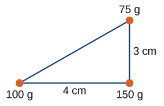
\includegraphics[width=0.35\textwidth]{graph_1.png} 
    % \label{fig:wrapfig}
\end{wrapfigure}
Figure 10-35 shows three 0.0100 kg particles that have been glued to a rod of length L = 6.00
cm and negligible mass. The assembly can rotate around a perpendicular axis through point O at
the left end. If we remove one particle (that is, 33\% of the mass), by what percentage does the
rotational inertia of the assembly around the rotation axis decrease when that removed particle
is (a) the innermost one and (b) the outermost one?

\subsection*{Solution}
\begin{align*}
    I_{123} &=  \Sigma m_i r_i^2
        =   10 * (2^2 + 4^2 + 6^2)
        =   10 * (4 + 16 + 36)
        =   10 * (56)
        =   560 \unit{\gram * \centi\meter^2}
\end{align*}

\textbf{a) 7.2\%}
\begin{align*}
    I_{23}  &=  10 * (4^2 + 6^2)
        =   10 * (16 + 36)
        =   10 * (52)
        =   520 \unit{\gram * \centi\meter^2}\\
    \frac{I_{23}}{I_{123}}  &=  \frac{520}{560}
        =   0.928
\end{align*}
The percentage lost is one minus the fraction, so the answer is $1 - \frac{I_{23}}{I_{123}} = 0.072 = \boxed{7.2\%}$.


\textbf{b) 64.3\%}
\begin{align*}
    I_{12}  &=  10 * (2^2 + 4^2)
        =   10 * (4 + 16)
        =   10 * (20)
        =   200 \unit{\gram * \centi\meter^2}\\
    \frac{I_{23}}{I_{123}}  &=  \frac{200}{560}
        =   0.357
\end{align*}
The percentage lost is one minus the fraction, so the answer is $1 - \frac{I_{12}}{I_{123}} = 0.643 = \boxed{64.3\%}$.


\pagebreak
\section*{Problem 2}
Two particles with masses 2.00 and 5.00 kg are connected by a light rod of length 2.00 m.
Find the moment of inertia of the system about an axis perpendicular to the rod and passing
through (a) the midpoint and (b) the center of mass.

\subsection*{Solution}
\subsubsection*{Section (a)}
We know that the midpoint of the rod is at 1 m. Mass constants allow us to calculate the moment of inertia without an integral.
\begin{align*}
    I   &=  \Sigma m_i r_i^2
        =   2 * (-1)^2 + 5 * 1^2
        =   2 + 5
        =   \boxed{7 \unit{\kilo\gram*\meter^2}}
\end{align*}

\subsubsection*{Section (b)}
We first calculate the center of mass.
\begin{equation*}
    x_{com} =   \frac{\Sigma_i m_i*r_i}{\Sigma m_i}
        =   \frac{2 * 0 + 5 * 2}{5 + 2}
        =   \frac{10}{7} \unit{\meter}
\end{equation*}
This means that the lighter mass will be located (relatively) at $-\frac{10}{7}$m, while the heavier mass will be located at $2 - \frac{10}{7} = \frac{4}{7}$m. We can calculate the moment of intertia from this.
\begin{equation*}
    I   =   2 * \left(-\frac{10}{7}\right)^2 + 5 * \left(\frac{4}{7}\right)^2
        =   2 * \frac{100}{49} + 5 * \frac{16}{49}
        =   \frac{200 + 80}{49}
        =   \boxed{\frac{280}{49} \unit{\kilo\gram*\meter^2}}
\end{equation*}

\pagebreak
\section*{Problem 3}
\begin{wrapfigure}{r}{0.35\textwidth}
    \vspace{-30pt}
    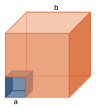
\includegraphics[width=0.35\textwidth]{graph_3.png} 
    % \label{fig:wrapfig}
\end{wrapfigure}
For each of the forces depicted in the figure find the torque about the pivot (black dot at
center of rod). Take $F_1$ = 10.0 N, $F_2$ = 15.0 N, $F_3$ = 8.00 N, and $L$ = 9.00 m. The 
rods length is L.

\subsection*{Solution}
Torque is calculatable with a sum. Torque is positive when counterclockwise and negative when clockwise.
\begin{align*}
    \tau    &=   \Sigma r_i F_i \sin(\phi)
        =   \frac{L}{2} F_1 \sin(60\unit{\degree}) + \frac{L}{4} F_2 \sin(-45\unit{\degree}) + \frac{L}{2} F_3\\
        &=  \frac{9*10\sqrt{3}}{4} - \frac{9*15*\sqrt{2}}{8} + \frac{8*9}{2}
        =   51.106\ \unit{\newton\cdot\meter}
\end{align*}
\begin{eqnarray*}
    \boxed{\tau_1 = \frac{45\sqrt{3}}{2}\ \unit{\newton\cdot\meter}}\\
    \boxed{\tau_2 = -\frac{135\sqrt{2}}{8}\ \unit{\newton\cdot\meter}}\\
    \boxed{\tau_3 = 36\ \unit{\newton\cdot\meter}}
\end{eqnarray*}

\pagebreak
\section*{Problem 4}
The angular position of a line on a disk of radius r = 6.00 cm is given by
\[ \theta = 10.0 - 5.00 t + 4 t^2\ \unit{\rad} \]
Find: (a) the average angular speed between 1.00 and 3.00 s; (b) the linear speed of a point on
the rim at 2.00 s; (c) the radial and tangential accelerations of a point on the rim at 2.00 s.

\subsection*{Solution}
\subsubsection*{Section (a)}
\begin{align*}
    \theta(1)   &=  10.0 - 5.00 * 1 + 4 * 1^2
        =   9\\
    \theta(3)   &=  10.0 - 5.00 * 3 + 4 * 3^2
        =   10 - 15 + 36
        =   31\\
    \omega_{avg}    &=  \frac{\theta(3) - \theta(1)}{3 - 1}
        =   \frac{31 - 9}{3 - 1}
        =   \frac{22}{2}
        =   \boxed{11\ \unit{\second^{-1}}}
\end{align*}

\subsubsection*{Section (b)}
\begin{align*}
    \omega(t)   &=  \frac{d\theta(t)}{dt}
        =   \frac{d}{dt}\left(10.0 - 5.00 t + 4 t^2\right)
        =   -5.00 + 8.00 t\\
    \omega(2)   &=  -5.00 + 8.00 * 2
        =   16 - 5
        =   11\ \unit{\second^{-1}}\\
    v_t(2)  &=  r*\omega(2)
        =   6*11
        =   \boxed{66\unit{\centi\meter/\second}}
\end{align*}

\subsubsection*{Section (c)}
\begin{align*}
    \alpha(t)   &=  \frac{d\omega(t)}{dt}
        =   \frac{d}{dt}\left(-5.00 + 8.00 t\right)
        =   8.00    \unit{\second^{-2}}\\
    a_t &=  r*\alpha
        =   6*8
        =   \boxed{48\unit{\centi\meter/\second^2}}\\
    a_c &=  \omega^2 r
        =   11^2*6
        =   121*6
        =   \boxed{726\unit{\centi\meter/\second^2}}
\end{align*}


\pagebreak
\section*{Problem 5}
\begin{wrapfigure}{r}{0.20\textwidth}
    \vspace{-30pt}
    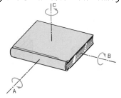
\includegraphics[width=0.20\textwidth]{graph_5.png} 
    % \label{fig:wrapfig}
\end{wrapfigure}
The book in the figure has the same shape as your physics textbook. About which axis is the
rotational inertia (a) the largest; (b) the smallest? \textit{You must justify your answer.}

\subsection*{Solution}
The rotational interia of any point is directly related to the mass and directly related to the square of the distance from the axis of rotation. Along any axis, we eliminate one dimension of any point's distance to the axis of rotation. No matter what axis we rotate around, the number of points and their masses will remain the same.\\
a) For the largest inertia, we should try to maximize the distance to the axis of rotation. Along axis C, we maximize the distance to any point by eliminating the smallest dimension of the object from rotation. This makes \boxed{C} the answer.\\
b) For the smallest inertia, we should try to minimize the distance to the axis of rotation. Along axis B, we minimize the distance to any point by eliminating the largest dimension of the object from rotation. This makes \boxed{B} the answer.



\pagebreak
\section*{Problem 6}
\begin{wrapfigure}{r}{0.30\textwidth}
    \vspace{-30pt}
    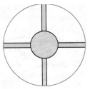
\includegraphics[width=0.30\textwidth]{graph_6.png} 
    % \label{fig:wrapfig}
\end{wrapfigure}
The wheel shown in the figure below has a central hub of radius 2.00 m and a mass of 2.00
kg. Each of the four spokes is 4.00 m long and has a mass of 1.00 kg. The outer thin ring has a
radius of 6.00 m and a mass of 2.00 kg. Find the rotational inertia about an axis through the
center perpendicular to the plane of the wheel. Treat the hub as a disk. \textit{Hint, you will have to
use the parallel axis theorem with the spokes.}

\subsection*{Solution}
We know the rotational inertia formula is \(I = \int r^2 dm\). We can assume all the components of the whole object to be of constant density. This means that the total inertia is equialent to the inertia of all the objects added together.
\[ I = I_{hub} + 4 I_{spoke} + I_{ring} \]
The axis of the hub and the ring are at the center of mass, but the axis of the spokes is not. For this, we can use the parallel-axis theorem, \(I = I_{com} + Mh^2\). For this, we also need to find the distance between the center of mass and the center of rotation. This would be half the length of the rod plus the radius of the hub, or \(h = \frac{L_{spoke}}{2} + r_{hub}\). This means that we can set up an equation for the total inertia and substitute in formulas for inertias.
\begin{align*}
    I   &=  I_{hub} + 4 I_{spoke} + I_{ring}
        =   I_{hub} + 4 I_{rod} + 4M_{spoke}h^2 + I_{ring}\\
        &=  \frac{1}{2}M_{hub}r_{hub}^2 + \frac{1}{3}M_{spoke}L_{spoke}^2 + 4M_{spoke}\left(\frac{L_{spoke}}{2} + r_{hub}\right)^2 + M_{ring}R_{ring}^2\\
        &=  \frac{1}{2}*2*2^2 + \frac{1}{3}*1*4^2 + 4*1\left(\frac{4}{2} + 2\right)^2 + 2*6^2\\
        &=  4 + \frac{16}{3} + 64 + 72
        =   140+\frac{16}{3}
        =   \boxed{\frac{436}{3} \unit{\kilo\gram*\meter^2} \approx 145.\bar{3} \unit{\kilo\gram*\meter^2}}
\end{align*}


\pagebreak
\section*{Problem 7}
\begin{wrapfigure}{r}{0.35\textwidth}
    \vspace{-30pt}
    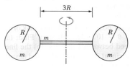
\includegraphics[width=0.35\textwidth]{graph_7.png} 
    % \label{fig:wrapfig}
\end{wrapfigure}
Two solid spheres of mass $m$ and radius $R$ are stuck to the ends of a thin rod of mass $m$ and
length $3R$. Find the rotational inertia of the system about the axis at the midpoint of the rod and
perpendicular to it, as shown in the figure below.

\subsection*{Solution}
We here use the formula for inertia and the parallel axis theorem. We then use the formula for the moment of inertia of a sphere and a rod to find our ultimate and final answer.
\begin{align*}
    I   &=  I_{rod} + 2I_{sphere}\\
    I_{rod} &=  \frac{1}{12}ML^2
        =   \frac{1}{12}m*(3R)^2
        =   \frac{3}{4}mR^2
        =   \frac{15}{20}mR^2\\
    I_{sphere}  &=  I_{sphere;com} + Mh^2
        =   \frac{2}{5}mR^2 + m*\left(\frac{5}{2}R\right)^2\\
        &=  \frac{8}{20}mR^2 + \frac{25}{4}mR^2
        =   \frac{133}{20}mR^2\\
    I   &=  \frac{15}{20}mR^2 + \frac{266}{20}mR^2
        =   \boxed{\frac{281}{20}mR^2}
\end{align*}


\pagebreak
\section*{Problem 8}
\begin{wrapfigure}{r}{0.35\textwidth}
    \vspace{-30pt}
    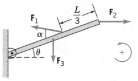
\includegraphics[width=0.35\textwidth]{graph_8.png} 
    % \label{fig:wrapfig}
\end{wrapfigure}
A light (massless) rod of length L = 1.5 m is freely pivoted at one end. Three forces act as
shown in the figure below. The force $\vec{F}_3$ acts at the midpoint. What is the torque due to each force?
Take $F_1$ = 6.90 N, $F_2$ = 4.00 N, $F_3$ = 2.00 N, $\theta = 20\unit{\degree}$, and $\alpha = 30\unit{\degree}$.

\subsection*{Solution}
\subsubsection{$F_1$}
\begin{align*}
    \tau_1  &=  F*r*\sin(\phi)
        =   F_1 * \frac{2L}{3} * \sin(\alpha)\\
        &=  6.90 * \frac{1.5*2}{3} * \sin(30\unit{\degree})
        =   6.90 * 1 * \frac{1}{2}
        =   \boxed{3.45 \unit{\newton*\meter}}
\end{align*}

\subsubsection{$F_2$}
\begin{align*}
    \tau_2  &=  F*r*sin(\phi)
        =   F_2 * L * \sin(-\theta)\\
        &=  4.00 * 1.5 * \sin(-20\unit{\degree})
        =   6 * (-0.342)
        =   \boxed{-2.052 \unit{\newton*\meter}}
\end{align*}

\subsubsection{$F_3$}
\begin{align*}
    \tau_3  &=  F * r * \sin(\phi)
        =   F_3 * \frac{L}{2} * \sin(\theta - 90\unit{\degree})\\
        &=  2.00 * \frac{1.5}{2} * \sin(-70\unit{\degree})
        =   1.5 * (-0.940)
        =   \boxed{-1.410 \unit{\newton*\meter}}
\end{align*}


\end{document}